\documentclass[a4paper, 11pt,reqno]{article}
\input{/Users/olivierglorieux/Desktop/BCPST/2020:2021/preambule.tex}
\usepackage{enumitem}
\geometry{hmargin=2.0cm, vmargin=2.5cm}
\lstset{basicstyle=\ttfamily, keywordstyle=\rmfamily\bfseries}
\newif\ifshow
\showtrue
\input{/Users/olivierglorieux/Desktop/BCPST/2021:2022/ifshow.tex}

\author{Olivier Glorieux}


\begin{document}

\title{Correction - DS 5
}
\begin{exercice}
Calculer
\begin{enumerate}
\item  $I_1=\ddp\int_1^2 \frac{\ln(t)}{t}dt$
\item $I_2 =\ddp \int_0^1 xe^{2x}dx$
\item $I_3 =\ddp\int_0^1 \frac{t}{1+t^4}dt$.\quad   (On pourra effectuer le changement de variable $t^2=u$.)
\end{enumerate}
\end{exercice}

\begin{correction}
\begin{enumerate}
\item  TD 10, ex 4, Q5
\item  TD 10, ex 5, Q2
\item  TD 10, ex 7, Q1
\end{enumerate}
\end{correction}
\vspace{0.5cm}

\begin{exercice}
Soit $f  : \R^2 \tv \R^2 $ définie par 
$$f(x,y)=(2x+y,  3x+y)$$

\begin{enumerate}
\item Soit $A = \begin{pmatrix}
2 & 1\\
3 & 1\\
\end{pmatrix}$. Montrer que $A$ est inversible et calculer son inverse. 

\item Justifier que pour tout $(X,Y)\in \R^2$ il existe une unique solution à l'équation d'inconnue $(x,y)$ : $$f(x,y)=(X,Y)$$
\item En déduire que $f$ est bijective et donner sa bijection réciproque. 
\end{enumerate}

\end{exercice}

\begin{correction}
\begin{enumerate}
\item On peut calculer le discriminant de $A$ ($ad-bc$) qui vaut $2-3=-1\neq 0$ donc $A$ est inversible et 
$$A^{-1} = \begin{pmatrix}
-1 & 1\\
3& -2
\end{pmatrix}$$
\item L'équation $f(x,y)=(X,Y)$ correspond à l'équation matricielle : 
$$A \begin{pmatrix}
x\\
y
\end{pmatrix}= \begin{pmatrix}
X\\
Y
\end{pmatrix}$$
Comme $A$ est inversible cette équation à une unique solution à savoir 
$$ \begin{pmatrix}
x\\
y
\end{pmatrix}= A^{-1}\begin{pmatrix}
X\\
Y
\end{pmatrix} = \begin{pmatrix}
-X+Y\\
3X-2Y
\end{pmatrix}$$
\item La question précédente signifie exactement que $f$ est bijective et 
\conclusion{$f^{-1} : (X,Y) \mapsto (-X+Y, 3X-2Y)$}
\end{enumerate}
\end{correction}

\vspace{0.5cm}


\begin{exercice}
\begin{enumerate}
\item Justifier que l'intégrale $\ddp \int_x^{2 x} \frac{1}{\sqrt{t^2+1}} d t$ est définie pour tout réel $x$.\\
On considère désormais la fonction $f$ définie par :
$$
\forall x \in \mathbb{R}, f(x)=\int_x^{2 x} \frac{1}{\sqrt{t^2+1}} d t
$$
\item  Etablir que $f$ est impaire. (Afin de caculer $f(-x)$, on pourra effectuer le changement de variable $t=-u$)
\item \begin{enumerate}
\item Justifier que $f$ est  dérivable  sur $\mathbb{R}$.
\item Montrer que pour tout $x\in \R$ :
$f'(x) $ est du signe de $\varphi(x)= 2\sqrt{x^2+1} -\sqrt{4x^2+1}$. 
\item Résoudre l'équation $\varphi(x)\geq 0$.
\item  En déduire que $f$ est strictement croissante sur $\mathbb{R}$.
\end{enumerate}
\item 
\begin{enumerate}
\item En utilisant la relation $t^2 \leqslant t^2+1 \leqslant t^2+2 t+1$, valable pour tout $t$ réel positif ou nul, montrer que l'on a l'encadrement suivant :
$$
\forall x \in \mathbb{R}_{+}^*, \quad \ln (2 x+1)-\ln (x+1) \leqslant f(x) \leqslant \ln (2)
$$
\item Donner alors la limite de $f(x)$ lorsque $x$ tend vers $+\infty$.
\item Dresser le tableau de variation complet de $f$.
\end{enumerate}
\item En déduire que $f$ est une bijection de $\R$ sur un ensemble à déterminer. 
\item Déterminer $f^{-1} (0) $ et  $(f^{-1})' (0)$.
\end{enumerate}
\end{exercice}
\begin{correction}
\begin{enumerate}
\item La fonction $t\mapsto \frac{1}{\sqrt{t^2+1}}$ est continue sur $\R$ donc admet une primitive, ainsi l'intégrale est bien définie pour tout $x\in \R$.
\item Soit $x\in \R$, calculons $f(-x)$ 
On a 
\begin{align*}
f(-x) &= \int_{-x}^{-2x} \frac{1}{\sqrt{t^2+1}} dt\\
\end{align*}
En faisant le changement de variable $u=-t$ on obtient 
\begin{itemize}
\item $\frac{1}{\sqrt{t^2+1}} = \frac{1}{\sqrt{u^2+1}} $.
\item $ dt=-du$.
\item Enfin les bornes sont envoyées sur $[x,2x]$.
\end{itemize}
On a donc : 
\begin{align*}
f(-x) &= \int_{x}^{2x} \frac{1}{\sqrt{u^2+1}}-du\\
	&= -\int_{x}^{2x} \frac{1}{\sqrt{u^2+1}}du\\
	&=-f(x)
\end{align*}
\conclusion{ $f$ est impaire}
\item 
\begin{enumerate}


\item Soit $G$ une primitive de $t\mapsto \frac{1}{\sqrt{t^2+1}}$, par définition $G$ est dérivable et $f(x) =G(2x) -G(x)$. Donc 
\conclusion{$f$ est dérivable sur $\R$}
\item On calcule la dérivée de $f$ à l'aide de la relation précédente on obtient 
$$f'(x) =2 G'(2x)-G'(x)$$
Or par défintion de $G$ on a  $G'(x)= \frac{1}{\sqrt{x^2+1}}$
Donc 
$$f'(x)= 2  \frac{1}{\sqrt{(2x)^2+1}}- \frac{1}{\sqrt{x^2+1}}$$

En mettant au même dénominateur on obtient 
$$f'(x) = \frac{2\sqrt{x^2+1} -\sqrt{4x^2+1} }{\sqrt{(2x)^2+1}\sqrt{x^2+1}}$$

\conclusion{ 
Le dénominateur étant positif le signe de $f'(x)$ est égal au signe de 
$2\sqrt{x^2+1} -\sqrt{4x^2+1}$
}


\item On résout : 
$(E) : \quad 2\sqrt{x^2+1} -\sqrt{4x^2+1}\geq 0$
On a 
\begin{align*}
(E)& \equivaut  2\sqrt{x^2+1}  \geq \sqrt{4x^2+1}
\end{align*}
Les deux cotés de l'inégalités étant positif on peut passer au carré et on a 
\begin{align*}
(E)& \equivaut  2^2(x^2+1)  \geq 4x^2+1\\
& \equivaut  4(x^2+1)  \geq 4x^2+1\\
& \equivaut  4 \geq 1
\end{align*}
Ainsi pour tout $x\in \R$, l'équation $E$ est vérifiée
\conclusion{ $\forall x\in \R, \phi(x) \geq 0$}


\item On vient de voir que $f'(x) $ était strictement positif sur $\R$ donc 
\conclusion{ $f$ est strictement croissante sur $\R$}
\end{enumerate}

\item 
\begin{enumerate}
\item A l'aide de l'encadrement donné on obtient, par décroissance de la fonction inverse sur $\R_+$ que pour tout $t\geq 0$:
$$\frac{1}{t^2}\geq \frac{1}{t^2+1}\geq \frac{1}{t^2+2t+1}$$
et donc en prenant la racine ( remarquons que $t^2+2t+1 = (t+1)^2)$
$$\frac{1}{t}\geq \frac{1}{\sqrt{t^2+1}}\geq \frac{1}{t+1}$$
Par croissance de l'intégrale on a alors (comme $x<2x$ car $x>0$ ) 
$$\int_x^{2x} \frac{1}{t}dt\geq \int_x^{2x}\frac{1}{\sqrt{t^2+1}}dt\geq\int_x^{2x} \frac{1}{t+1}dt$$
On peut alors intégrer les différents membres de l'inégalité pour obtenir : 
$$[\ln(t)]_x^{2x} \geq f(x) \geq [\ln(t+1)]_x^{2x}$$
D'où 
$$\ln(2x)-\ln(x) \geq f(x) \geq \ln(2x+1)-\ln(x+1)$$
ce qui donne  (car $\ln(2x)-\ln(x)=\ln(2)$) : 
\conclusion{  $\ln(2x+1)-\ln(x+1)\leq f(x) \leq \ln(2)$}

\item $\ln(2x+1)-\ln(x+1) = \ln\left( \frac{2x+1}{x+1}\right)$. 
Or $\lim_{x\tv +\infty} \frac{2x+1}{x+1} =2 $ donc par composition de limite 
$$\lim_{x\tv +\infty } \ln(2x+1)-\ln(x+1) =\ln(2)$$

On applique ensuite le théorème d'encadrement et on a 
\conclusion{ $\lim_{x\tv +\infty } f(x) =\ln(2)$}


\item On obtient le tableau de variation suivant à l'aide de l'imparité de $f$ et de la question précédente. 
\begin{center}
\begin{tikzpicture}
   \tkzTabInit{$x$ / 1 , $f(x)$ / 1.5}{$-\infty $,$+\infty$}
   \tkzTabVar{-/ $-\ln(2)$, +/ $\ln(2)$}
\end{tikzpicture}
\end{center}

\item $f$ est continue (car dérivable) et strictement croissante, de plus $\lim_{x\tv +\infty} f(x)= \ln(2)$ et  $\lim_{x\tv -\infty} f(x)= -\ln(2)$

\conclusion{Le théorème de la bijection assure que $f$ réalise une bijection de $\R$ sur $]-\ln(2) , \ln(2)[$}

\item $f(0) = \int_0^0 \frac{1}{\sqrt{t^2+1}}dt=0$ 
Dont $$f^{-1} (0) =0$$

Pour calculer $(f^{-1} )'(0)$ il suffit d'appliquer la formule de dérivation de la bijection réciproque : 
$$(f^{-1})'(0) =\frac{1}{f'\circ f^{-1}(0) }$$
On a par ailleurs: 
$f'\circ f^{-1}(0) = f'(f^{-1}(0)) = f'(0) = 2\frac{1}{\sqrt{2\times 0)^2 +1 }  }- \frac{1}{\sqrt{\times 0)^2 +1 }  }=1$

\conclusion{ $(f^{-1})'(0) =1$}

\end{enumerate}
\end{enumerate}


\end{correction}

\vspace{0.5cm}
\newpage

\begin{exercice}
Soit $M$ la matrice : 
$$M=\left( \begin{array}{ccc}
2 &1& 0\\
0 &1 & 0  \\
 -1&0&1
\end{array}\right) $$

\begin{enumerate}
%\item  Résoudre le système $MX=\lambda X$ d'inconnue $X =\left(
%\begin{array}{c}
%x\\
%y\\
%z
%\end{array}
% \right)$ où $\lambda$ est un paramètre réel. 
\item Calculer $(M- \Id)^2$. Donner son rang.

 \item Soit $e_1= \left(
\begin{array}{c}
1\\
0\\
-1
\end{array}
 \right)$,  $e_2= \left(
\begin{array}{c}
0\\
0\\
1
\end{array}
 \right)$, et  $e_3= \left(
\begin{array}{c}
1\\
-1\\
0
\end{array}
 \right)$.
Exprimer  $Me_1, Me_2$ en fonction de $e_1, e_2$.
\item Montrer qu'il existe $(\alpha, \beta)\in \R^2$ tel que $M e_3 = \alpha e_2 +\beta e_3$.
 
\item Soit $P= \left(
\begin{array}{ccc}
1&0&1\\
0&0&-1\\
-1&1&0
\end{array}
 \right)$ 
 
 Montrer que $P$ est inversible et calculer son inverse. 
 \item Soit $T=P^{-1}MP$. Calculer $T$. 
  \item Montrer par récurrence que 
$$T^n = \left(\begin{array}{ccc}  
2^n&0&0 \\
0 &1&-n \\
0&0&1 
\end{array}\right)$$
 \item Montrer par récurrence que pour tout $n\in \N$: 
 $$T^n = P^{-1}M^n P$$
\item En déduire la valeur de $M^n$.
\item Soit $\suite{x}, \suite{y}, \suite{z}$ trois suites telles que $x_0=1, y_0=2, z_0=-1$ et $\forall n\in \N$
$$\left\{ \begin{array}{ccc}
x_{n+1} &=& 2x_n+y_n\\
y_{n+1} &= & y_n\\
z_{n+1} &= & -x_n+z_n\\
\end{array}\right.$$
\begin{enumerate}
\item On pose $U_n =\left(\begin{array}{c}
x_n\\
y_n\\
z_n
\end{array}   \right)$. Etablir une relation entre $U_n, U_{n+1}$ et $M$.
\item En déduire  (et la prouver) une relation entre $U_n$ $U_0$ et $M$
\item Donner finalement l'expression de $x_n$ en fonction de $n$. 
\end{enumerate}

\end{enumerate}
\end{exercice}

\vspace{3cm}
\begin{center}
Dernier exercice page suivante.
\end{center}


\begin{correction}
\begin{enumerate}
%\item
%$$MX=\lambda X \equivaut   \left( \begin{array}{c}
%2x +y  \\
% y \\
% -x +z
%\end{array}\right) = \left(
%\begin{array}{c}
%\lambda x\\
%\lambda y\\
%\lambda z
%\end{array} \right)$$ 
%
%$$\left\{ \begin{array}{ccccc}
%2x &+y& & =&\lambda x \\
% &y & & =& \lambda y \\
% -x& &+z&=&\lambda z
%\end{array}\right. 
%\equivaut \left\{ \begin{array}{ccccc}
%(2-\lambda)x &+y& & =&0 \\
% &(1-\lambda)y & & =& 0 \\
% -x& &+(1-\lambda)z&=&0
%\end{array}\right. 
%$$ 
% En échangeant les lignes et les colonnes on peut voir que le système est déjà échelonné.
%$L_3\leftarrow L_1, L_2 \leftarrow _3, L_1\leftarrow L_2$
%$$MX=\lambda X 
%\equivaut  \left\{ \begin{array}{ccccc}
% -x& &+(1-\lambda)z&=&0\\
%(2-\lambda)x &+y& & =&0 \\
% &(1-\lambda)y & & =& 0 
%\end{array}\right.$$
%$ C_3\leftarrow C_1, C_2 \leftarrow C_3, C_1\leftarrow C_2$
%$$
%\equivaut \left\{ \begin{array}{ccccc}
% (1-\lambda)z&-x& &=&0\\
% &(2-\lambda)x&+y & =&0 \\
% &  & (1-\lambda)y& =& 0 
%\end{array}\right.$$
%
%Si $\lambda \notin \{ 1,2\} $ alors le système est de rang 3, il est donc de Cramer et l'unique solution est 
%\conclusion{ $\cS= \{ (0,0,0)\}$}
%
%Si $\lambda =1$, le système est équivalent à 
%$$\left\{ \begin{array}{cccc}
% -x& &=&0\\
% (2-1)x&+y & =&0 \\
%   & 0& =& 0 
%\end{array}\right. \equivaut \left\{ \begin{array}{cc}
% x& =0\\
% y&  =0
%\end{array}\right.$$
%Le système est de rang 2. L'ensemble des solutions est 
%\conclusion{ $\cS= \{ (0,0,z) \, |\, z\in \R\}$}
%
%Si $\lambda =2$, le système est équivalent à 
%$$\left\{ \begin{array}{ccccc}
%(1-2)z&-x& &=&0\\
% & 0 &+y & =&0 \\
% &  & (1-2)y& =& 0 
%\end{array}\right. \equivaut \left\{ \begin{array}{cccc}
%-z&-x& &=0\\
% &  &y  &=0 \\
% &  & y &= 0 
%\end{array}\right.\equivaut \left\{ \begin{array}{cl}
%x &=-z\\
%  y  &=0 
%\end{array}\right.$$
%Le système est de rang 2. L'ensemble des solutions est 
%\conclusion{ $\cS= \{ (-z,0,z) \, |\, z\in \R\}$}
%
\item $M-\Id= \left( \begin{array}{ccc}
1 &1& 0\\
0 &0& 0  \\
 -1&0&0
\end{array}\right) $

Donc \conclusion{$(M-\Id)^2= \left( \begin{array}{ccc}
1 &1& 0\\
0 &0& 0  \\
 -1&-1&0
\end{array}\right) $}

Le système associé est 

$\left\{  \begin{array}{ccr}
x &+y&  =0\\
 & & 0  =0\\
 -x&-y&=0
\end{array}\right. \equivaut \left\{  \begin{array}{cr}
x +y&  =0\\
\end{array}\right. $
Il est de rang 1. Donc
\conclusion{$(M-\Id)^2$ est de rang $1$}
\item 
Le calcul montre que $Me_1 =2e_1$ et  $Me_2=e_2$
\item Le calcul montre que 
$Me_3 =  \left( \begin{array}{c}
1\\
-1\\
-1\\
\end{array}\right) = \left( \begin{array}{c}
1\\
-1\\
0\\
\end{array}\right) - \left( \begin{array}{c}
0\\
\\
1\\
\end{array}\right)  e_3-e_2 $


Ainsi on peut prendre 
\conclusion{$\alpha =-1$ et $\beta =1$}

\item  On considère la matrice augmentée : 
$\left(\begin{array}{ccc|ccc}  
1&0&1 & 1&0&0 \\
0&0&-1& 0&1&0 \\
-1&1&0& 0&0&1 
\end{array}\right)$

$L_3\leftarrow L_3+L_1$  donnent
$$\left(\begin{array}{ccc|ccc}  
1&0&1 & 1&0&0 \\
0&0&-1& 0&1&0 \\
0&1&1& 1&0&1 
\end{array}\right)$$
$L_1\leftarrow L_1+L_2$ et $L_3\leftarrow L_3+L_2$
donne 
$$\left(\begin{array}{ccc|ccc}  
1&0&0 & 1&1&0 \\
0&0&-1& 0&1&0 \\
0&1&0& 1&1&1 
\end{array}\right)$$

$L_2\leftarrow -L_2$
donne 
$$\left(\begin{array}{ccc|ccc}  
1&0&0 & 1&1&0 \\
0&0&1& 0&-1&0 \\
0&1&0& 1&0&1 
\end{array}\right)$$
Enfin 
$L_2\leftrightarrow L_3$
donne 
$$\left(\begin{array}{ccc|ccc}  
1&0&0 & 1&1&0 \\
0&1&0& 1&1&1 \\
0&0&1& 0&-1&0 
\end{array}\right)$$

\conclusion{ $P$ est inversible d'inverse $\left(\begin{array}{ccc}  
1&1&0 \\
 1&1&1 \\
0&-1&0 
\end{array}\right)$}

\item Le calcul donne  
\conclusion{ $T=\left(\begin{array}{ccc}  
2&0&0 \\
0 &1&-1 \\
0&0&1 
\end{array}\right)$}
(sur une copie, le produit intermédiaire $MP$ serait apprécié)

\item
Soit $Q(n) $ la propriété $'T^n=\left(\begin{array}{ccc}  
2^n&0&0 \\
0 &1&-n \\
0&0&1 
\end{array}\right)'$

\begin{itemize}
\item \emph{Initialisation} $T^0=I_3$ et en remplacant on obtient 
$\left(\begin{array}{ccc}  
2^0&0&0 \\
0 &1&-0 \\
0&0&1 
\end{array}\right) =I_3$
Donc $Q(0)$ est vraie.

\item Hérédité On suppose que la propriété $Q(n) $ est vraie pour un certain entier $n$ on a donc $T^n =\left(\begin{array}{ccc}  
2^n&0&0 \\
0 &1&-n \\
0&0&1 
\end{array}\right)$, donc 
$$T^{n+1} = \left(\begin{array}{ccc}  
2^n&0&0 \\
0 &1&-n \\
0&0&1 
\end{array}\right) \left(\begin{array}{ccc}  
2&0&0 \\
0 &1&-1 \\
0&0&1 
\end{array}\right)$$
Le calcul donne 
$$T^{n+1} = \left(\begin{array}{ccc}  
2^{n+1}&0&0 \\
0 &1&-{n+1} \\
0&0&1 
\end{array}\right) $$

La proposition $Q(n+1)$ est vraie. 
\item Conclusion $Q(n) $ est vraie pour tout $n\in \N$. 

\end{itemize}

\item 




On pose $P(n) : "T^n =P^{-1} M^n P"$
\begin{itemize}
\item[Initialisation] 
$T^1 =T$ et $P^{-1} M^1 P= P^{-1} M P=T$ d'après la définition de $T$.
Donc $P(1) $ est vrai. 

\item[Hérédité] On suppose qu'il existe $n\in \N$ tel que $P(n)$ soit vraie. 
On a alors 
\begin{align*}
 (T)^{n+1}&=  T^n  T
\end{align*}
et donc par Hypothése de récurrence : 
\begin{align*}
 T^{n+1}&=  (P^{-1}M^n P )  (P^{-1}M P )\\
 							&=  (P^{-1}M^n P  P^{-1}M P )\\
 							&=  (P^{-1}M^n \Id M P )\\
 							&=  (P^{-1}M^n M P )\\
 							&=  (P^{-1}M^{n+1} P )
\end{align*}
\item[Conclusion] $P(n)$ est vraie pour tout $n$. 




\end{itemize}
\item 
D'après la question précédente : 
$M^n = PT^n P^{-1}$. Tout calcul fait on obtient : 
\conclusion{
 $M^n=\left(\begin{array}{ccc}  
2^n&2^n-1&0 \\
0&1&0 \\
-2^n+1&-2^n+1+n&1 
\end{array}\right)$

}

\item \begin{enumerate}
\item Le système correspond à 
\conclusion{ $U_{n+1}=M U_n$}

\item
On pose $P(n) : "U_n = M^n U_0"$
\begin{itemize}
\item[Initialisation] 
$P(0):  "U_0 = M^0 U_0" \equivaut  "U_0 = I_3 U_0" \equivaut  "U_0 =  U_0"$
donc $P(0)$ est vraie. 

\item[Hérédité] On suppose qu'il existe $n\in \N$ tel que $P(n)$ soit vraie. 
On a alors 
\begin{align*}
U_n=M^n U_0
\end{align*}
Donc $MU_n= M \times M^{n}U_0$ et d'après la question précédente $U_{n+1} =MU_n$ donc 
$$U_{n+1} =M^{n+1} U_0$$
La propriété $P(n+1)$ est donc vérifiée. 
\item[Conclusion] $P(n)$ est vraie pour tout $n$. 




\end{itemize}
\item Il suffit de réaliser la multiplication entre $M^n $ et $U_0$. On obtient 
$$x_n = 2^n -2(2^n-1) +1\times 0 = -2^n+2$$
\conclusion{ $\forall n\in \N, x_n=-2^n +2$}

\end{enumerate}




\end{enumerate}
\end{correction}


\begin{exercice}

\begin{enumerate}

\item On consid\`ere la chaine de caract\`ere \verb|ch = "1234"|.

\begin{enumerate}

\item Quel est le type de \verb|ch[0]| ? Quelle est sa valeur ?
\item Quel est le type de \verb|int(ch[3])| ? Quelle est sa valeur ?
\item Quel est le type de \verb|"1" + str(2)| ? Quelle est sa valeur ?

\end{enumerate}

\item \'Ecrire une fonction \verb|StringToList| qui prend comme argument d'entrée une chaine de caractères repr\'esentant un nombre entier positif (de longueur quelconque) et qui renvoie la liste des chiffres qui composent l'entier repr\'esent\'e par la chaine de caract\`eres.

\textit{Par exemple, l'instruction }\verb|StringToList("1234")| \textit{renverra la liste d'entiers }\verb|[1, 2, 3, 4]|.
\item \'Ecrire une fonction \verb|distribution| qui, \`a partir d'une liste d'entiers compris entre $0$ et $9$, renvoie une liste \verb|L| telle que, pour tout $i\in\llbracket0,9\rrbracket$, \verb|L[i]| contienne le nombre d'entiers \verb|i| dans la liste pass\'ee en argument.

\textit{Par exemple, }\verb|distribution([4, 7, 7, 1])| r\textit{enverra la liste} \verb|[0, 1, 0, 0, 1, 0, 0, 2, 0, 0]|.
\item On consid\`ere une fonction \verb|NbEntiersCommuns| qui renvoie le nombre d'entiers en commun (mais pas n\'ecessairement plac\'es aux m\^eme endroit) dans deux listes d'entiers (compris entre $0$ et $9$) pass\'ees en argument.

\textit{Par exemple,} \verb|NbEntiersCommuns([4, 7, 7, 1], [4, 4, 7, 7])| \textit{renverra $3$.}

Parmis les fonctions suivantes, indiquer (sans justifier) l'unique fonction qui correspond \`a celle d\'ecrite ci-dessus.

\begin{minipage}{.45\textwidth}
\begin{lstlisting}[language=Python]
def NbEntiersCommuns1(L,M) :
    s = 0
    for k in range(len(L)) :
        s += min(L[k], M[k])
    return s
\end{lstlisting}
\begin{lstlisting}[language=Python]
def NbEntiersCommuns3(L,M) :
    nb = 0
    for k in range(len(L)) :
        i = 0
        while i < len(M) :
            if L[k] == M[i] :
                nb = nb + 1
    return nb
\end{lstlisting}
\end{minipage}
\hspace{.5cm}
\begin{minipage}{.45\textwidth}
\begin{lstlisting}[language=Python]
def NbEntiersCommuns2(L,M) :
    nb = 0
    dL = distribution(L)
    dM = distribution(M)
    for k in range(10) :
        nb += max(dL[k], dM[k])
    return nb
\end{lstlisting}
\begin{lstlisting}[language=Python]
def NbEntiersCommuns4(L,M) :
    s = 0
    dL = distribution(L)
    dM = distribution(M)
    for k in range(10) :
        s += max(dL[k], dM[k])
    return s
\end{lstlisting}
\end{minipage}

%\item \'Ecrire une fonction \verb|NbEntiersCommunsCh| qui renvoie le nombre d'entiers en commun (mais pas n\'ecessairement plac\'es aux m\^eme endroit) dans deux chaines de caract\`eres repr\'esentant un entiers (compris entre $0$ et $9$) pass\'ees en argument.
%
%\textit{Par exemple,} \verb|NbEntiersCommunsCh("4771", "4477")| \textit{renverra $3$.}

\end{enumerate}

\end{exercice}

\end{document}